\section{Robot architecture}

A machine gathers information from a set of sensors and utilizes this data to autonomously execute tasks by controlling its body parts.

One commonly employed model in robotics is the sense plan act paradigm, which forms the foundation of cognitive robotics.
In this model, the sensing phase involves collecting data from sensors, the planning phase utilizes algorithms to process this data, and the action phase involves executing commands through actuators.
This architecture is illustrated in the following diagram.

\begin{figure}[H]
    \centering
    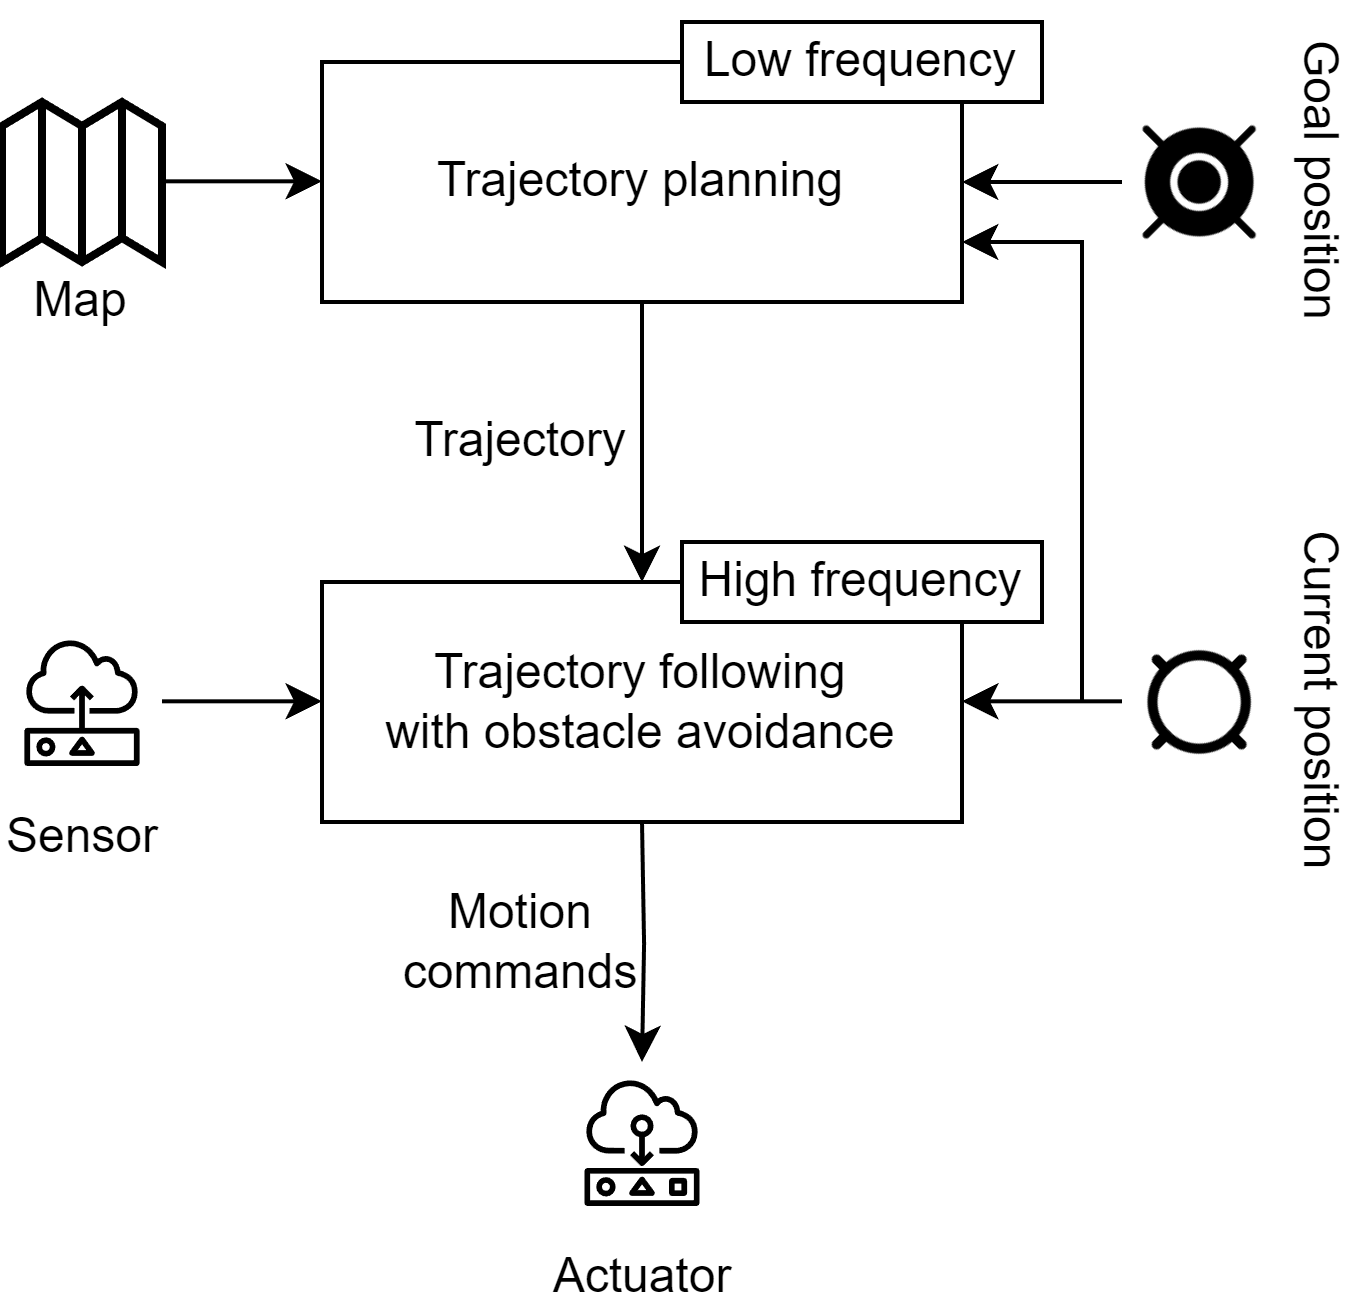
\includegraphics[width=0.6\linewidth]{images/sap.png}
    \caption{Sense plan act architecture}
\end{figure}